
\documentclass[a4paper,10pt]{article}


\usepackage{graphicx}
\usepackage{float}
\usepackage{amsmath}
\usepackage{color}


\usepackage[latin1]{inputenc}

\usepackage[spanish]{babel}



\title{		\textbf{Trabajo Pr�ctico Final}}


\author{	Bruno, Tom�s ; \textit{Padr�n Nro. 88.449}                     \\
            \texttt{ tbruno88@gmail.com }                                              \\
			Ferreiro, Demian ; \textit{Padr�n Nro. }                     \\
            \texttt{ epidemian@gmail.com }                                              \\	
			Leguizamo, Mat�as ; \textit{Padr�n Nro. }                     \\
            \texttt{ matias.leguizamo@gmail.com }                                              \\	
            Mouso, Nicol�s ; \textit{Padr�n Nro. 88.528}                     \\
            \texttt{ nicolasgnr@gmail.com }                                              \\[2.5ex]
            \normalsize{1er. Cuatrimestre de 2010}                       \\
            \normalsize{75.10 Tecnicas de Dise�o}                             \\
            \normalsize{Facultad de Ingenier�a, Universidad de Buenos Aires}            \\
       }
\date{}



\begin{document}

% Inserta el t�tulo.
\maketitle

% Quita el n�mero en la primer p�gina.
\thispagestyle{empty}


\clearpage
\tableofcontents

\clearpage
\section{Hipot�sis}
	\begin{enumerate}
		\item Las m�quinas se pueden reparar por separado o se puede reparar toda una l�nea al mismo tiempo
		\item Se pueden romper tanto las m�quinas de control de calidad como las que son 
			exclusivamente para la producci�n.
		\item Las maquinas pueden levantarse o no con una entrada y una salida determinada. 
			En caso de que no tengan una establecida entonces se les genera una por defecto.
		\item Tanto los precios de la materia prima como los de los productos var�an todas las 
			semanas. El resto de los precios se mantiene invariante en el tiempo
		\item Las paredes no pueden ser borradas del terreno adquirido.
	\end{enumerate}

\clearpage
\section{Vista L�gica}
	\subsection{Producci�n}
		
		%La estructura de la producci�n es el esqueleto de todo el juego. 
		
		\textcolor{red}{Explicacion acerca de: raw materials, product guarda history. Hace falta describir una a una las clases?}	
		
		\begin{figure}[H]
		\centering
		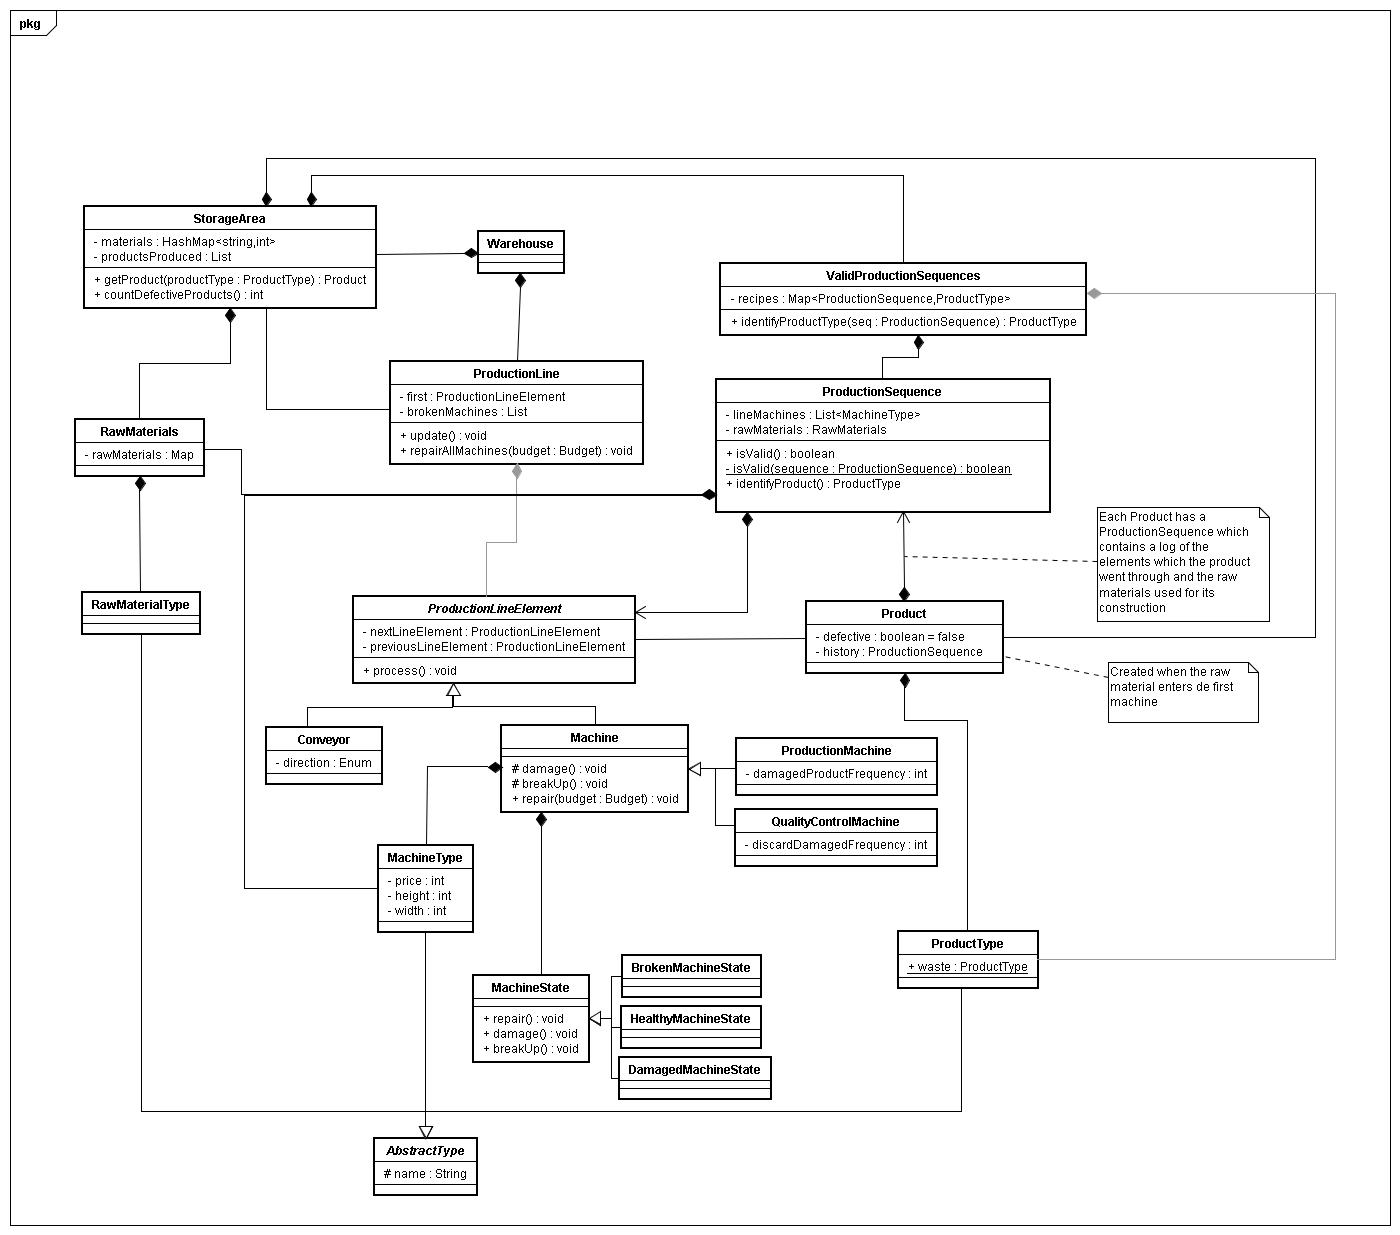
\includegraphics[scale=0.25]{diagramas/productionClassDiagram.jpg}
		\caption{Diagrama de Clases de la l�gica de producci�n}
		\end{figure}		
	
		\begin{figure}[H]
		\centering
		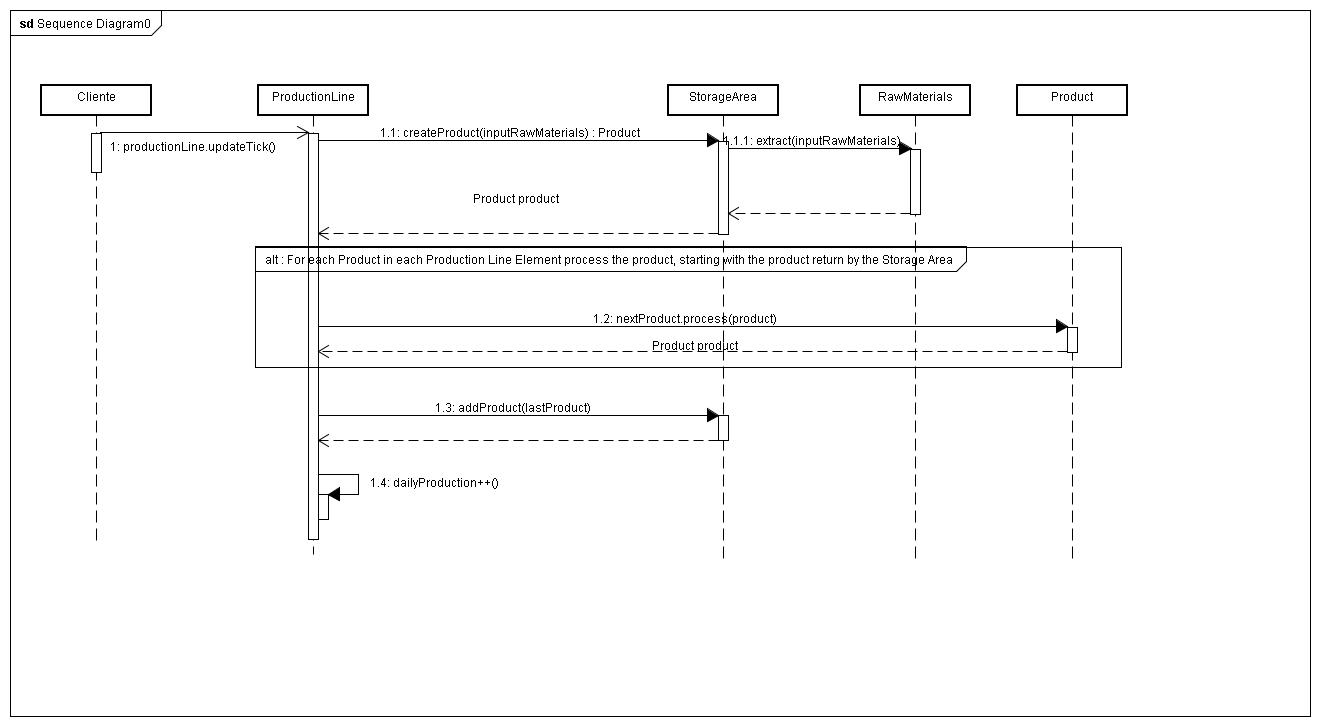
\includegraphics[scale=0.3]{diagramas/productionSequenceDiagram.jpg}
		\caption{Diagrama de Secuencia de la l�gica de producci�n}
		\end{figure}		
				
	\subsection{Tecnolog�a }
		
		\begin{figure}[H]
		\centering
		\includegraphics[scale=0.3]{diagramas/TechnologyClassDiagram.jpg}
		\caption{Diagrama de Clases de la l�gica del desarrollo de Tecnolog�as}
		\end{figure}	
		
\clearpage
\section{Vista de Procesos}
	\textcolor{red}{mmm... la bibliografia dice de usar diagrama de actividades, o de estados. Pero...}	

\clearpage
\section{Vista de Desarrollo}
				
	
	
	\begin{figure}[H]
	\centering
	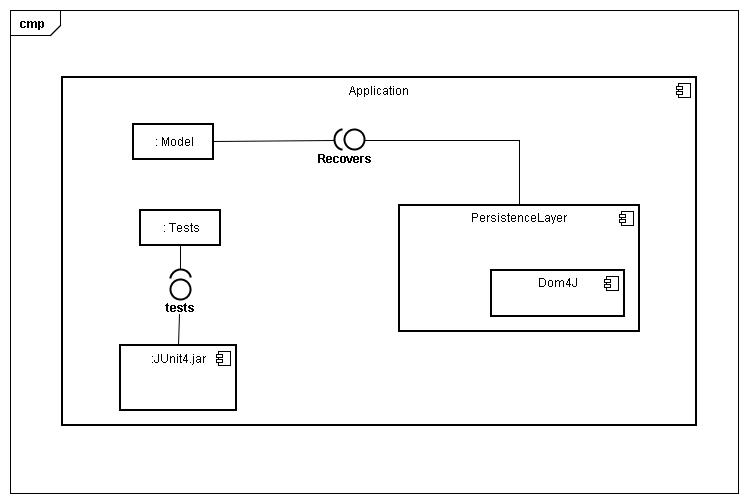
\includegraphics[scale=0.5]{diagramas/componentDiagram.jpg}
	\caption{Diagrama de Componentes}
	\end{figure}
	
	\subsection{Componentes}
		
	\textcolor{red}{Breve descripcion acerca de cada componente}	
	
\clearpage
\section{Vista F�sica}
	\begin{figure}[H]
	\centering
	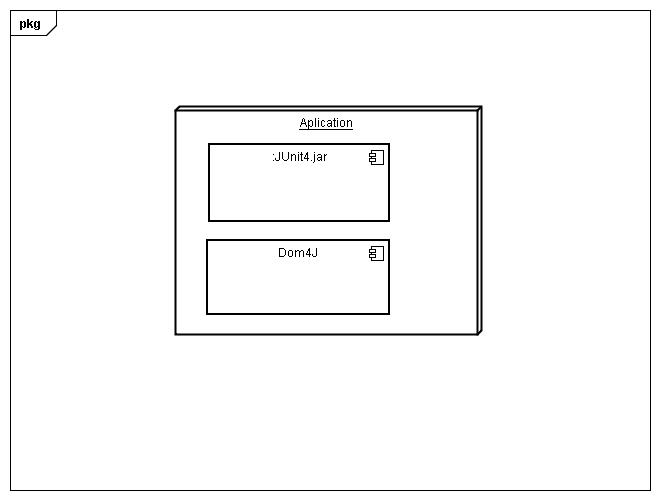
\includegraphics[scale=0.5]{diagramas/deployment.jpg}
	\caption{Diagrama de Emplazamiento }
	\end{figure}
	
\clearpage
\section{Escenarios}
	
	\textcolor{red}{Completar CUs}	

	\begin{figure}[H]
	\centering
	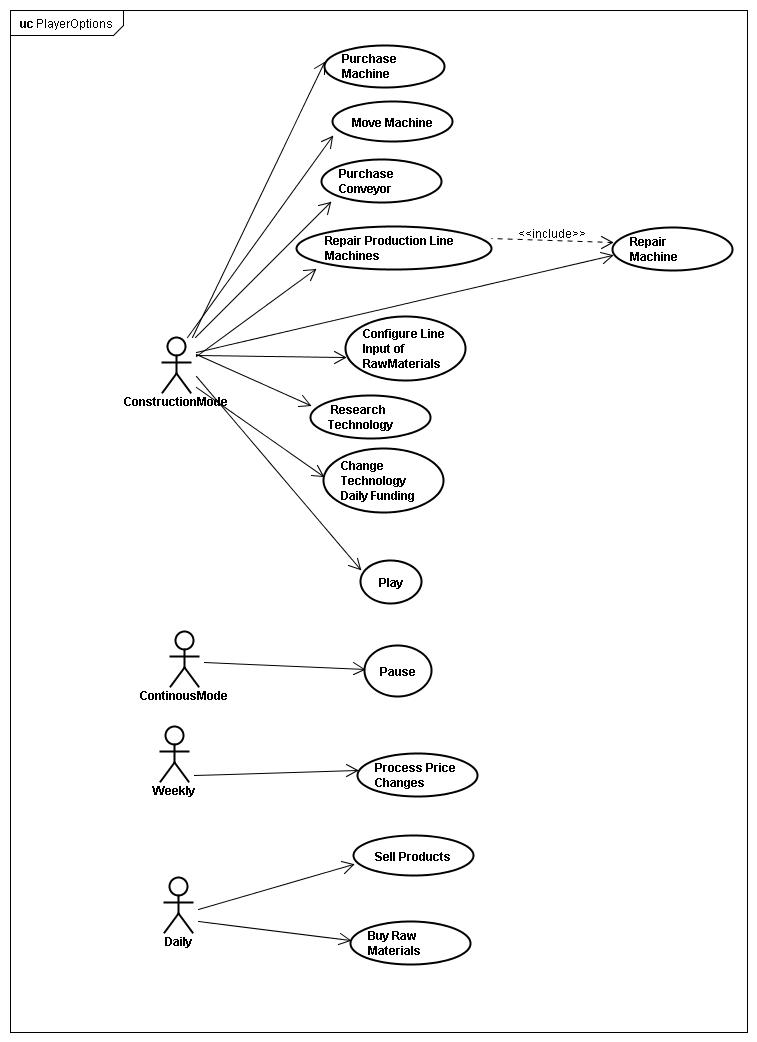
\includegraphics[scale=0.5]{diagramas/useCase.jpg}
	\caption{Diagrama de Casos de Uso}
	\end{figure}			
	
	\subsection{Funcionalidades}
	
		\textcolor{red}{Breve descripcion acerca de cada CU}	
	
		\begin{enumerate}
			\item{\emph{ :}}
			\item{\emph{ :}}
			\item{\emph{ :}}
			\item{\emph{ :}}
			\item{\emph{ :}}
		\end{enumerate}
	
\clearpage
\begin{thebibliography}{9}
  \bibitem{ieee} KRUCHTEN, Philipe. ``Architectural Blueprints $\-$ The \emph{4+1} View Model of Software Architecture''
  \bibitem{wiki} Wikipedia EN, ``4+1 Architectural View Model''
\end{thebibliography}

\end{document}

